\documentclass[11pt]{article}

\usepackage{xltxtra}
\setromanfont{Libertinus Serif}
\setsansfont{Libertinus Sans}
\usepackage{polyglossia}
\setdefaultlanguage{english}
\usepackage[autostyle]{csquotes}

\usepackage{verbatim}
\usepackage{url}


\usepackage[
    sorting=none,  % Sort in citation oder, better for the reviews
    backend=biber,
    % backend=bibtex,
    % style=authoryear-icomp,
    % % style=alphabetic,
    % dashed=false,
    % sortlocale=en_us,
    % firstinits=true,
    giveninits=true,
    % terseinits=false,
    % maxcitenames=2,
    % block=none, %space?
    % natbib=false,
     % url=false, 
    % doi=false,
    % isbn=false,
    % eprint=false,
]{biblatex}

\addbibresource{zib_challenge.bib}
 
\usepackage[a4paper]{geometry}
% \geometry{a4paper, left=4cm, right=4cm, top=3.5cm}  %, top=20mm}
% \geometry{a4paper, top=2.5cm, bottom=2.5cm}

\title{ZIB Challenge}
\author{David Nolte}
\date{\today}

\begin{document}

\maketitle

\section*{Docker containers}

Two \verb!docker! containers are created and connected via a \verb!docker!
network: one container holding the database (\verb!MongoDB!, populated by the
script \verb!docker_db/populate_db.py!) and the other containing the
\verb!JupyterLab!  environment for deep neural networks (with
\verb!tensorflow/keras!) and the notebooks for solving the given task (see
folder \verb!docker_jl!).

The repository's \verb!README.rst! explains the procedure.

\section*{ECG Dataset}
The dataset is a subset of the large ECG signal PTB-XL data
set \cite{wagner_ptb-xl_2020}, considering only
those ECG timeseries where the cardiac rhythm diagnosis was marked \emph{sinus
    rhythm} (SR) or \emph{atrial fibrillation} (AFIB).
The dataset is partitioned into 10 folds, where the first 8 are recommended
by the authors of \cite{wagner_ptb-xl_2020} for the training of a neural network, and 9 and 10---the
data with the highest confidence in the diagnosis---for testing and validation.
All timeseries are normalized such that their be 0 and the standard deviation be 1.

\section*{Deep Neural Network}
A deep neural network is trained to classify the ECG time series into `SR' and
`AFIB'. A residual neural network (ResNet) is used, following
\cite{kachuee_ecg_2018,spdrnl_ecg_2021}.
The implementation uses the \verb!keras! library.
See the code in the \verb!jupyter! notebook \verb!ecg_resnet.ipynb! and the
references \cite{kachuee_ecg_2018,spdrnl_ecg_2021} for details on the setup.
Conveniently, this setup can be run on an old laptop without GPUs.


\section*{Results}
The accuracy of the ResNet w.r.t.\ the training and the validation data over 75
training iterations is illustrated in Fig.~\ref{fig:accu}.
\begin{figure}[htpb]
    \centering
    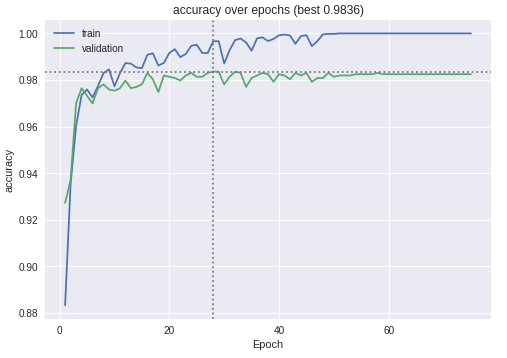
\includegraphics[width=0.8\linewidth]{accuracy}
    \caption{ResNet accuracy with training data}%
    \label{fig:accu}
\end{figure}

The test dataset is classified with an accuracy of 0.9787.
A useful metric for the quality of the trained network is the confusion matrix,
showing the number of correctly and erroneously classified sets, see
Fig.~\ref{fig:conf}.
\begin{figure}[htpb]
    \centering
    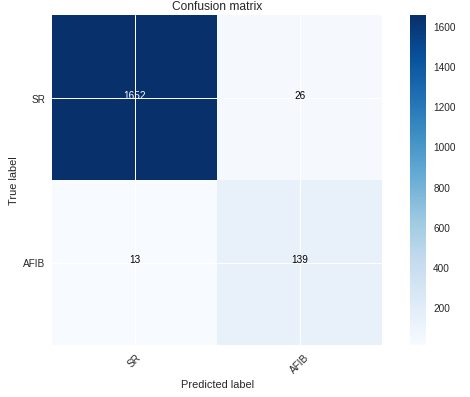
\includegraphics[width=0.8\linewidth]{confusion}
    \caption{Confusion matrix for testing dataset}%
    \label{fig:conf}
\end{figure}
26 ECG signals labelled SR are wrongly
classified as AFIB, and 13 AFIB data are wrongly predicted as SR.

\printbibliography

\end{document}
